% Options for packages loaded elsewhere
\PassOptionsToPackage{unicode}{hyperref}
\PassOptionsToPackage{hyphens}{url}
%
\documentclass[
]{article}
\usepackage{amsmath,amssymb}
\usepackage{iftex}
\ifPDFTeX
  \usepackage[T1]{fontenc}
  \usepackage[utf8]{inputenc}
  \usepackage{textcomp} % provide euro and other symbols
\else % if luatex or xetex
  \usepackage{unicode-math} % this also loads fontspec
  \defaultfontfeatures{Scale=MatchLowercase}
  \defaultfontfeatures[\rmfamily]{Ligatures=TeX,Scale=1}
\fi
\usepackage{lmodern}
\ifPDFTeX\else
  % xetex/luatex font selection
\fi
% Use upquote if available, for straight quotes in verbatim environments
\IfFileExists{upquote.sty}{\usepackage{upquote}}{}
\IfFileExists{microtype.sty}{% use microtype if available
  \usepackage[]{microtype}
  \UseMicrotypeSet[protrusion]{basicmath} % disable protrusion for tt fonts
}{}
\makeatletter
\@ifundefined{KOMAClassName}{% if non-KOMA class
  \IfFileExists{parskip.sty}{%
    \usepackage{parskip}
  }{% else
    \setlength{\parindent}{0pt}
    \setlength{\parskip}{6pt plus 2pt minus 1pt}}
}{% if KOMA class
  \KOMAoptions{parskip=half}}
\makeatother
\usepackage{xcolor}
\usepackage{color}
\usepackage{fancyvrb}
\newcommand{\VerbBar}{|}
\newcommand{\VERB}{\Verb[commandchars=\\\{\}]}
\DefineVerbatimEnvironment{Highlighting}{Verbatim}{commandchars=\\\{\}}
% Add ',fontsize=\small' for more characters per line
\newenvironment{Shaded}{}{}
\newcommand{\AlertTok}[1]{\textcolor[rgb]{1.00,0.00,0.00}{\textbf{#1}}}
\newcommand{\AnnotationTok}[1]{\textcolor[rgb]{0.38,0.63,0.69}{\textbf{\textit{#1}}}}
\newcommand{\AttributeTok}[1]{\textcolor[rgb]{0.49,0.56,0.16}{#1}}
\newcommand{\BaseNTok}[1]{\textcolor[rgb]{0.25,0.63,0.44}{#1}}
\newcommand{\BuiltInTok}[1]{\textcolor[rgb]{0.00,0.50,0.00}{#1}}
\newcommand{\CharTok}[1]{\textcolor[rgb]{0.25,0.44,0.63}{#1}}
\newcommand{\CommentTok}[1]{\textcolor[rgb]{0.38,0.63,0.69}{\textit{#1}}}
\newcommand{\CommentVarTok}[1]{\textcolor[rgb]{0.38,0.63,0.69}{\textbf{\textit{#1}}}}
\newcommand{\ConstantTok}[1]{\textcolor[rgb]{0.53,0.00,0.00}{#1}}
\newcommand{\ControlFlowTok}[1]{\textcolor[rgb]{0.00,0.44,0.13}{\textbf{#1}}}
\newcommand{\DataTypeTok}[1]{\textcolor[rgb]{0.56,0.13,0.00}{#1}}
\newcommand{\DecValTok}[1]{\textcolor[rgb]{0.25,0.63,0.44}{#1}}
\newcommand{\DocumentationTok}[1]{\textcolor[rgb]{0.73,0.13,0.13}{\textit{#1}}}
\newcommand{\ErrorTok}[1]{\textcolor[rgb]{1.00,0.00,0.00}{\textbf{#1}}}
\newcommand{\ExtensionTok}[1]{#1}
\newcommand{\FloatTok}[1]{\textcolor[rgb]{0.25,0.63,0.44}{#1}}
\newcommand{\FunctionTok}[1]{\textcolor[rgb]{0.02,0.16,0.49}{#1}}
\newcommand{\ImportTok}[1]{\textcolor[rgb]{0.00,0.50,0.00}{\textbf{#1}}}
\newcommand{\InformationTok}[1]{\textcolor[rgb]{0.38,0.63,0.69}{\textbf{\textit{#1}}}}
\newcommand{\KeywordTok}[1]{\textcolor[rgb]{0.00,0.44,0.13}{\textbf{#1}}}
\newcommand{\NormalTok}[1]{#1}
\newcommand{\OperatorTok}[1]{\textcolor[rgb]{0.40,0.40,0.40}{#1}}
\newcommand{\OtherTok}[1]{\textcolor[rgb]{0.00,0.44,0.13}{#1}}
\newcommand{\PreprocessorTok}[1]{\textcolor[rgb]{0.74,0.48,0.00}{#1}}
\newcommand{\RegionMarkerTok}[1]{#1}
\newcommand{\SpecialCharTok}[1]{\textcolor[rgb]{0.25,0.44,0.63}{#1}}
\newcommand{\SpecialStringTok}[1]{\textcolor[rgb]{0.73,0.40,0.53}{#1}}
\newcommand{\StringTok}[1]{\textcolor[rgb]{0.25,0.44,0.63}{#1}}
\newcommand{\VariableTok}[1]{\textcolor[rgb]{0.10,0.09,0.49}{#1}}
\newcommand{\VerbatimStringTok}[1]{\textcolor[rgb]{0.25,0.44,0.63}{#1}}
\newcommand{\WarningTok}[1]{\textcolor[rgb]{0.38,0.63,0.69}{\textbf{\textit{#1}}}}
\usepackage{longtable,booktabs,array}
\usepackage{calc} % for calculating minipage widths
% Correct order of tables after \paragraph or \subparagraph
\usepackage{etoolbox}
\makeatletter
\patchcmd\longtable{\par}{\if@noskipsec\mbox{}\fi\par}{}{}
\makeatother
% Allow footnotes in longtable head/foot
\IfFileExists{footnotehyper.sty}{\usepackage{footnotehyper}}{\usepackage{footnote}}
\makesavenoteenv{longtable}
\usepackage{graphicx}
\makeatletter
\def\maxwidth{\ifdim\Gin@nat@width>\linewidth\linewidth\else\Gin@nat@width\fi}
\def\maxheight{\ifdim\Gin@nat@height>\textheight\textheight\else\Gin@nat@height\fi}
\makeatother
% Scale images if necessary, so that they will not overflow the page
% margins by default, and it is still possible to overwrite the defaults
% using explicit options in \includegraphics[width, height, ...]{}
\setkeys{Gin}{width=\maxwidth,height=\maxheight,keepaspectratio}
% Set default figure placement to htbp
\makeatletter
\def\fps@figure{htbp}
\makeatother
\setlength{\emergencystretch}{3em} % prevent overfull lines
\providecommand{\tightlist}{%
  \setlength{\itemsep}{0pt}\setlength{\parskip}{0pt}}
\setcounter{secnumdepth}{-\maxdimen} % remove section numbering
\ifLuaTeX
  \usepackage{selnolig}  % disable illegal ligatures
\fi
\IfFileExists{bookmark.sty}{\usepackage{bookmark}}{\usepackage{hyperref}}
\IfFileExists{xurl.sty}{\usepackage{xurl}}{} % add URL line breaks if available
\urlstyle{same}
\hypersetup{
  hidelinks,
  pdfcreator={LaTeX via pandoc}}

\author{}
\date{}

\begin{document}

\section{Classifying Concord}

\label{classifying-concord}

© 2025 Richard Anton. All rights reserved.

\subsection{Introduction}\label{introduction}

This article is a walkthrough of using machine learning classification
techniques combined with some preprocessing to distinguish between the
writing of Emerson and Thoreau.

I wanted to show methods for classifying text using a novel dataset
rather than one of the toy ones so often used for tutorials. Eventually
I settled on classifying text to predict the original author. Since I
wanted this to be primarily about actual writing style rather than the
changes to language between regions or over time I chose two authors
from the same era and location, Emerson and Thoreau. For background on
computational authorship attribution see Koppel et al. (2009) .

\emph{Walden} has always been one of my favorite books and had a big
influence on me when I first read it in high school, but Emerson was a
different story. I found his writing style wordy and frustrating.
Recently I revisited the context of these works when I read
\emph{\href{https://us.macmillan.com/books/9780374279325/thetranscendentalistsandtheirworld/}{The
Transcendentalists and Their World}} (Gross, 2021) which gave me the
idea to use their writings as the basis for this project.

The dataset was created from two public domain works, one by each
author. For Emerson, I used \emph{Essays: First Series} (1841), and for
Thoreau, there was really no choice but \emph{Walden, and On The Duty Of
Civil Disobedience} (1854).

The texts were segmented into passages of 3-5 sentences each, creating a
collection of labeled examples for training and testing classification
models.

To explore how different machine learning approaches perform on this
task I compared multiple methods including classical models like logistic regression, random forests, and support vector machines, along with newer transformer-based models.

The accompanying code, but not this article itself, is licensed under the
MIT License. See the LICENSE file for details.

\subsection{The Evolution of Machine Learning
Classification}\label{the-evolution-of-machine-learning-classification}

Text classification has developed substantially over the years. Early
methods in the 1960s relied on hand-crafted rules, for example Rocchio
(1971), then statistical techniques took over. Advanced neural networks
joined simpler statistical models in the following years, notably
recurrent neural networks (Sebastiani, 2002). More recently,
transformer-based models have gained prominence in this and most other
natural language processing (NLP) use cases from 2018 onward.

\begin{enumerate}
\def\labelenumi{\arabic{enumi}.}
\item
  \textbf{Rule-based systems} (1960s-1980s): Manually crafted rules and
  decision trees.
\item
  \textbf{Statistical methods} (1990s-2000s): Naïve Bayes, Support
  Vector Machines, and Logistic Regression
\item
  \textbf{Neural network approaches} (2010s): Recurrent neural networks
  (RNNs) including LSTMs (Hochreiter \& Schmidhuber, 1997) and
  convolutional neural networks (CNNs) (LeCun et al. 1998).
\item
  \textbf{Transformer models} (2018-present): BERT, GPT, and their
  derivatives following the original "Attention is All You Need" paper
  on transformers Vaswani, A. et al., 2017).
\end{enumerate}

Each era brought improvements to accuracy and capability. The field also
expanded from simple categorization to include other use cases like
sentiment analysis, authorship attribution (Stamatatos, 2009), and
stylometry---the quantitative study of writing style (Burrows, 2002).

We compare methods across this range, first with TF-IDF representation with various classifiers then using a pretrained transformer DistilBERT model first as a feature extractor, then directly as a classifier with fine-tuning.

\subsection{Creating a Unique Literary
Dataset}\label{creating-a-unique-literary-dataset}

\subsubsection{Data Acquisition}\label{data-acquisition}

First, we selected two representative texts from Project
Gutenberg\textquotesingle s public domain collection.
(\href{https://www.gutenberg.org/}{Project Gutenberg}, n.d.).

\begin{Shaded}
\begin{Highlighting}[]
\NormalTok{emerson\_txt\_url }\OperatorTok{=} \StringTok{"https://www.gutenberg.org/ebooks/16643.txt.utf{-}8"}
\NormalTok{thoreau\_txt\_url }\OperatorTok{=} \StringTok{"https://www.gutenberg.org/ebooks/205.txt.utf{-}8"}

\KeywordTok{def}\NormalTok{ download\_file(url):}
\NormalTok{    local\_filename }\OperatorTok{=}\NormalTok{ Path(url.split(}\StringTok{\textquotesingle{}/\textquotesingle{}}\NormalTok{)[}\OperatorTok{{-}}\DecValTok{1}\NormalTok{])}
\NormalTok{    result }\OperatorTok{=}\NormalTok{ requests.get(url)}
\NormalTok{    result.raise\_for\_status()}
    \ControlFlowTok{with} \BuiltInTok{open}\NormalTok{(local\_filename, }\StringTok{"wb"}\NormalTok{) }\ImportTok{as}\NormalTok{ f:}
\NormalTok{        f.write(result.content)}
    \ControlFlowTok{return}\NormalTok{ local\_filename}
    
\NormalTok{emerson\_file }\OperatorTok{=}\NormalTok{ download\_file(emerson\_txt\_url)}
\NormalTok{thoreau\_file }\OperatorTok{=}\NormalTok{ download\_file(thoreau\_txt\_url)}
\end{Highlighting}
\end{Shaded}

This programmatic approach ensures reproducibility and automation eliminating the need for manual file handling.

\subsubsection{Text Preprocessing}\label{text-preprocessing}

Both works contain Project Gutenberg boilerplate text that needs
removal. We identify the start of the actual content by searching for
the standard "START OF THE PROJECT GUTENBERG EBOOK" marker:

\begin{Shaded}
\begin{Highlighting}[]
\KeywordTok{def}\NormalTok{ trim\_frontmatter(filename):}
    \ControlFlowTok{with} \BuiltInTok{open}\NormalTok{(filename) }\ImportTok{as}\NormalTok{ f:}
\NormalTok{        lines }\OperatorTok{=}\NormalTok{ f.readlines()}
\NormalTok{    n\_trim\_lines }\OperatorTok{=} \DecValTok{0}
    \ControlFlowTok{for}\NormalTok{ i, line }\KeywordTok{in} \BuiltInTok{enumerate}\NormalTok{(lines):}
        \ControlFlowTok{if} \StringTok{"START OF THE PROJECT GUTENBERG EBOOK"} \KeywordTok{in}\NormalTok{ line:}
\NormalTok{            n\_trim\_lines }\OperatorTok{=}\NormalTok{ i }\OperatorTok{+} \DecValTok{1}
            \ControlFlowTok{break}
\NormalTok{    trimmed\_lines }\OperatorTok{=}\NormalTok{ lines[n\_trim\_lines:]}
\NormalTok{    trimmed\_content }\OperatorTok{=} \StringTok{\textquotesingle{}}\CharTok{\textbackslash{}n}\StringTok{\textquotesingle{}}\NormalTok{.join(trimmed\_lines)}
\NormalTok{    new\_filename }\OperatorTok{=} \SpecialStringTok{f"trimmed\_}\SpecialCharTok{\{}\NormalTok{filename}\SpecialCharTok{\}}\SpecialStringTok{"}
    \ControlFlowTok{with} \BuiltInTok{open}\NormalTok{(new\_filename, }\StringTok{"w"}\NormalTok{) }\ImportTok{as}\NormalTok{ f:}
\NormalTok{        f.write(trimmed\_content)}
    \ControlFlowTok{return}\NormalTok{ new\_filename}
\end{Highlighting}
\end{Shaded}

\subsubsection{Text Segmentation}\label{text-segmentation}

We segment the texts into manageable chunks of 3-5 sentences each. This
creates a dataset with many examples for training and testing while
preserving enough context to capture authorial style. We did not directly experiment with different sample lengths, but having the variability allows us to still do some comparison on how the length affects model performance.

This function creates randomly-sized windows of 3-5 sentences, providing
natural text chunks while introducing variation in the dataset.

\begin{Shaded}
\begin{Highlighting}[]
\KeywordTok{def}\NormalTok{ segment\_doc(filename):}
    \ControlFlowTok{with} \BuiltInTok{open}\NormalTok{(filename) }\ImportTok{as}\NormalTok{ f:}
\NormalTok{        text }\OperatorTok{=}\NormalTok{ f.read()}
\NormalTok{    doc }\OperatorTok{=}\NormalTok{ nlp(text)}
    \ControlFlowTok{assert}\NormalTok{ doc.has\_annotation(}\StringTok{"SENT\_START"}\NormalTok{)}
\NormalTok{    sent\_dq }\OperatorTok{=}\NormalTok{ deque()}
\NormalTok{    n }\OperatorTok{=}\NormalTok{ randint(}\DecValTok{3}\NormalTok{, }\DecValTok{5}\NormalTok{)}
    \ControlFlowTok{for}\NormalTok{ sent }\KeywordTok{in}\NormalTok{ doc.sents:}
\NormalTok{        sent\_dq.append(sent)}
        \ControlFlowTok{if} \BuiltInTok{len}\NormalTok{(sent\_dq) }\OperatorTok{\textgreater{}}\NormalTok{ n:}
\NormalTok{            sent\_dq.popleft()}
\NormalTok{        snippet }\OperatorTok{=} \StringTok{" "}\NormalTok{.join(sent.text }\ControlFlowTok{for}\NormalTok{ sent }\KeywordTok{in}\NormalTok{ sent\_dq)}
        \ControlFlowTok{yield}\NormalTok{ snippet}
\NormalTok{        n }\OperatorTok{=}\NormalTok{ randint(}\DecValTok{3}\NormalTok{, }\DecValTok{5}\NormalTok{)}
\NormalTok{        sent\_dq.clear()}
\end{Highlighting}
\end{Shaded}

\subsubsection{Dataset Creation}\label{dataset-creation}

We create pandas DataFrames from these segments and label them with
their respective authors:

\begin{Shaded}
\begin{Highlighting}[]
\NormalTok{emerson\_df }\OperatorTok{=}\NormalTok{ dataframe\_from\_file(trimmed\_emerson\_file)}
\NormalTok{emerson\_df[}\StringTok{"label"}\NormalTok{] }\OperatorTok{=} \StringTok{"emerson"}

\NormalTok{thoreau\_df }\OperatorTok{=}\NormalTok{ dataframe\_from\_file(trimmed\_thoreau\_file)}
\NormalTok{thoreau\_df[}\StringTok{"label"}\NormalTok{] }\OperatorTok{=} \StringTok{"thoreau"}

\NormalTok{combined\_df }\OperatorTok{=}\NormalTok{ pd.concat([emerson\_df, thoreau\_df])}
\NormalTok{combined\_df }\OperatorTok{=}\NormalTok{ shuffle(combined\_df, random\_state}\OperatorTok{=}\DecValTok{7919}\NormalTok{)}
\end{Highlighting}
\end{Shaded}

The result is a dataset of 1,911 text segments (1,064 from Emerson and
847 from Thoreau), each labeled with its author. This is relatively balancd which helps prevent bias in the models.

\subsection{Overview of Methods}\label{overview-of-methods}

At a high level there are two versions of the ML pipeline whether we are
using a deep learning/transformers based approach or using a more
traditional path.

\textbf{Traditional path} (blue): Raw Text → Preprocessing → TF-IDF →
Classical ML models → Classification

\textbf{Transformer path} (green): Raw Text → Preprocessing → BERT
embeddings → Fine-tuned model → Classification

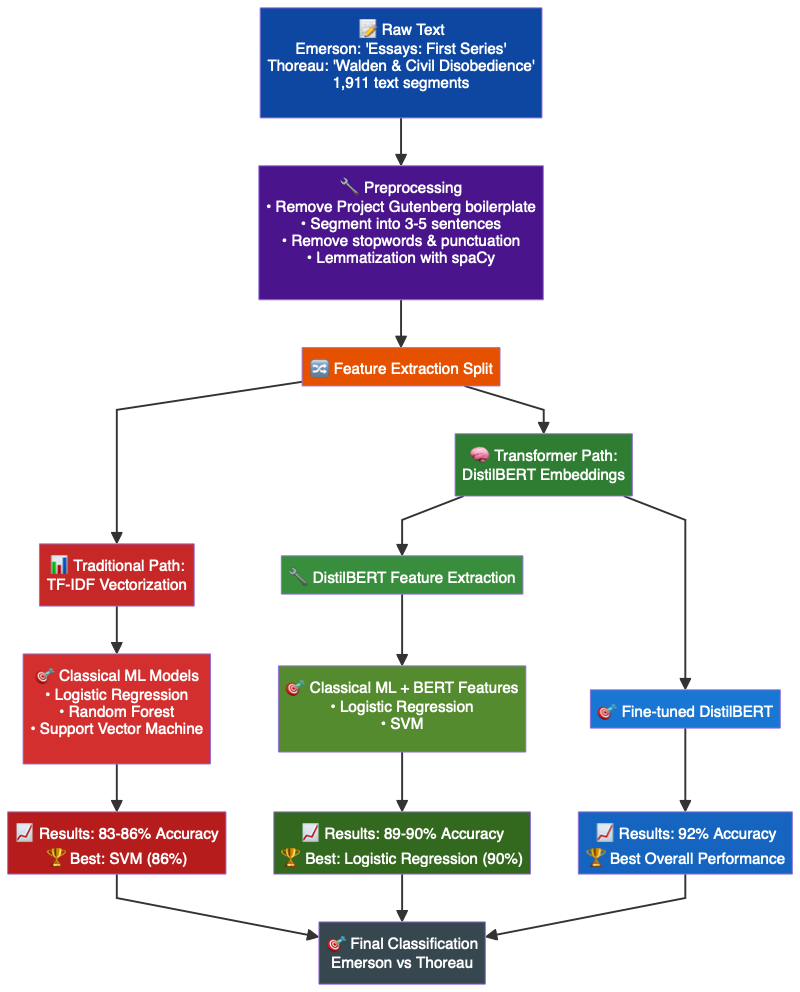
\includegraphics[width=8.33333in,height=\textheight]{image-20250611165131252.png}

\subsection{Text Representation
Techniques}\label{text-representation-techniques}

\subsubsection{Visualization with Word
Clouds}\label{visualization-with-word-clouds}

Before diving into classification, we visualize the most frequent words
used by each author through word clouds, excluding common stopwords:

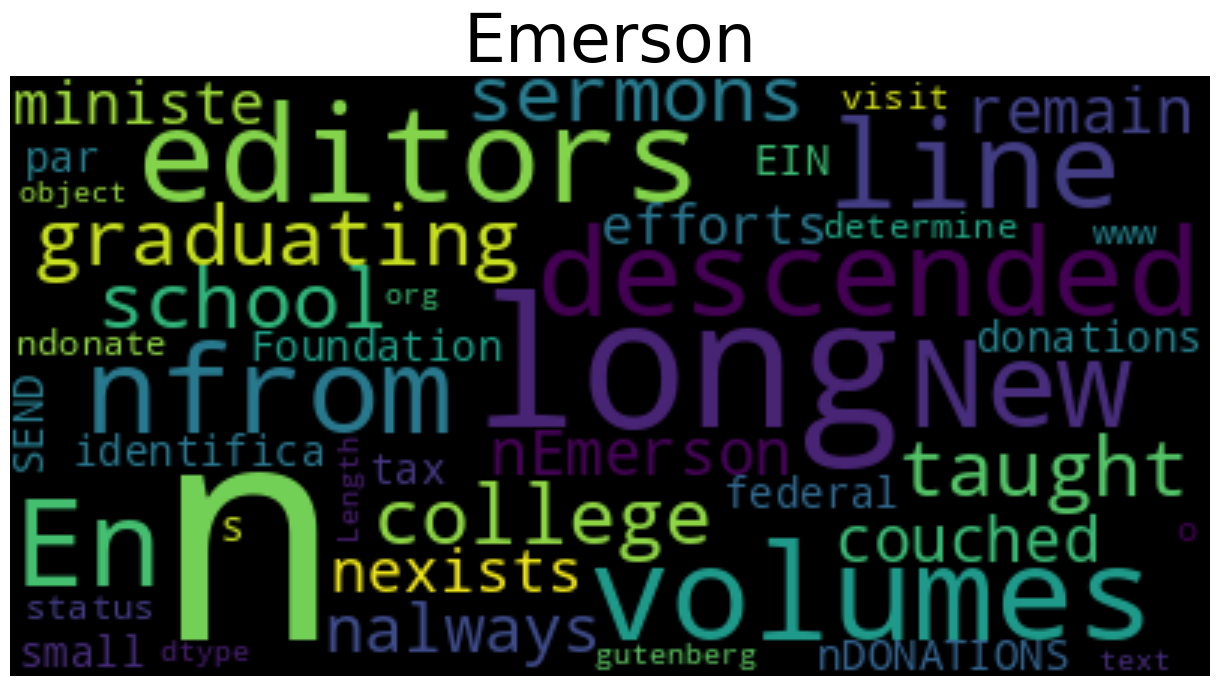
\includegraphics{emerson_word_cloud.png}

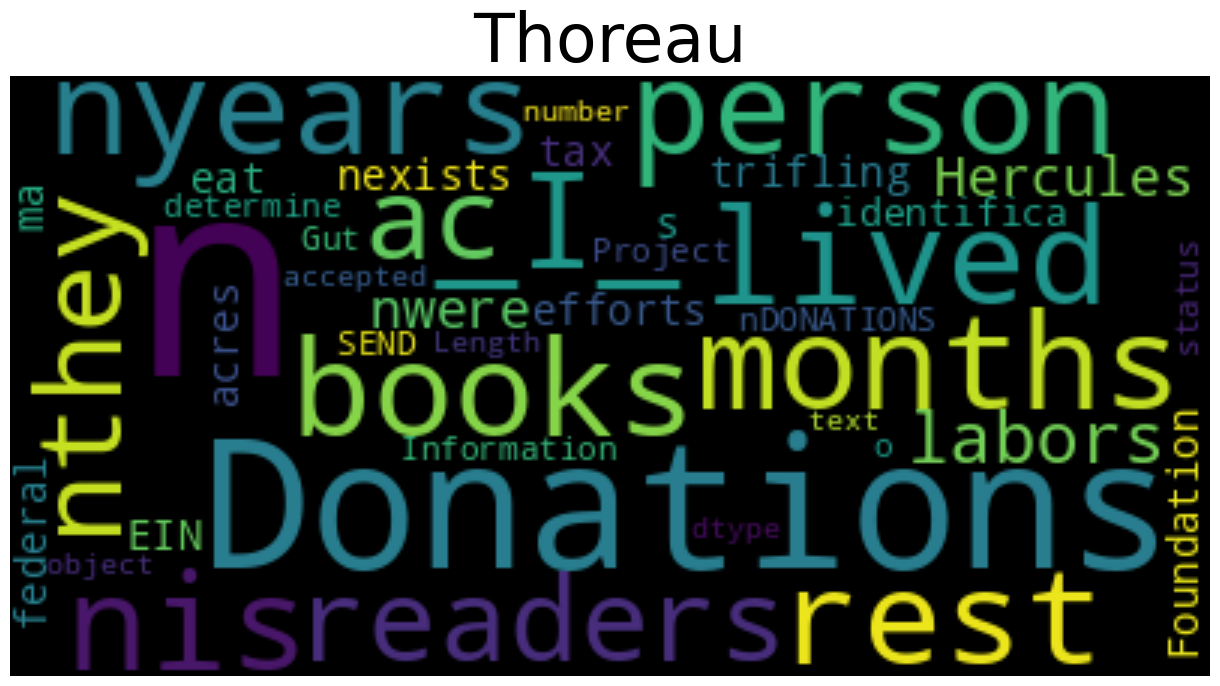
\includegraphics{thoreau_word_cloud.png}

These visualizations already reveal interesting differences in
vocabulary. Emerson\textquotesingle s text prominently features abstract
terms like "soul," "nature," "truth," and "power," reflecting his focus
on philosophical concepts. Thoreau\textquotesingle s cloud emphasizes
more concrete words like "house," "wood," "water," and "life," mirroring
his practical observations at Walden Pond.

\subsubsection{Text Preprocessing for
ML}\label{text-preprocessing-for-ml}

We preprocess the text using \href{https://spacy.io/}{spaCy} (Honnibal \& Montani, 2017) to remove stopwords and perform lemmatization, which reduces words to their base forms:

\begin{Shaded}
\begin{Highlighting}[]
\NormalTok{final\_text }\OperatorTok{=}\NormalTok{ []}
\ControlFlowTok{for}\NormalTok{ index, entry }\KeywordTok{in} \BuiltInTok{enumerate}\NormalTok{(combined\_df[}\StringTok{\textquotesingle{}text\textquotesingle{}}\NormalTok{]):}
\NormalTok{    doc }\OperatorTok{=}\NormalTok{ nlp(entry.lower())}
\NormalTok{    Final\_words }\OperatorTok{=}\NormalTok{ []}
    \ControlFlowTok{for}\NormalTok{ word }\KeywordTok{in}\NormalTok{ doc:}
        \ControlFlowTok{if} \KeywordTok{not}\NormalTok{ word.is\_stop }\KeywordTok{and} \KeywordTok{not}\NormalTok{ word.is\_punct:}
\NormalTok{            Final\_words.append(word.lemma\_)}
\NormalTok{    final\_text.append(}\StringTok{\textquotesingle{} \textquotesingle{}}\NormalTok{.join(Final\_words))}

\NormalTok{combined\_df[}\StringTok{\textquotesingle{}final\_text\textquotesingle{}}\NormalTok{] }\OperatorTok{=}\NormalTok{ final\_text}
\end{Highlighting}
\end{Shaded}

\subsubsection{TF-IDF Vectorization}\label{tf-idf-vectorization}

For our traditional machine learning models, we convert text to
numerical features using Term Frequency-Inverse Document Frequency
(\href{https://en.wikipedia.org/wiki/Tf–idf}{TF-IDF}) vectorization:

\begin{Shaded}
\begin{Highlighting}[]
\NormalTok{vectorizer }\OperatorTok{=}\NormalTok{ TfidfVectorizer()}
\NormalTok{X }\OperatorTok{=}\NormalTok{ vectorizer.fit\_transform(combined\_df[}\StringTok{"final\_text"}\NormalTok{])}
\NormalTok{y }\OperatorTok{=}\NormalTok{ combined\_df[}\StringTok{"label"}\NormalTok{]}
\end{Highlighting}
\end{Shaded}

TF-IDF converts text into numerical vectors by calculating two
components for each word: how frequently it appears in a specific
document (Term Frequency), and how unique it is across all documents
(Inverse Document Frequency) (Jones, 1972). The value combines how
frequently the term appears in the document (TF) and how unique it is
across all documents (IDF). This balances common words against
distinctive ones that might better differentiate the authors (Salton \&
Buckley, 1988).

\subsection{Traditional ML Classification
Models}\label{traditional-ml-classification-models}

We split our dataset into training (80\%) and test (20\%) sets to
evaluate model performance, as typically needed for a supervised ML workflow:

\begin{Shaded}
\begin{Highlighting}[]
\NormalTok{x\_train, x\_test, y\_train, y\_test }\OperatorTok{=}\NormalTok{ train\_test\_split(X, y, test\_size}\OperatorTok{=}\FloatTok{0.2}\NormalTok{, random\_state}\OperatorTok{=}\DecValTok{4909}\NormalTok{)}
\end{Highlighting}
\end{Shaded}

\subsubsection{Logistic Regression}\label{logistic-regression}

We begin with
\href{https://en.wikipedia.org/wiki/Logistic_regression}{logistic
regression}, a simple but effective linear classifier (Cox, D.R., 1958).

\begin{Shaded}
\begin{Highlighting}[]
\NormalTok{lr\_model }\OperatorTok{=}\NormalTok{ LogisticRegression(solver}\OperatorTok{=}\StringTok{\textquotesingle{}saga\textquotesingle{}}\NormalTok{, random\_state}\OperatorTok{=}\DecValTok{8102}\NormalTok{, n\_jobs}\OperatorTok{={-}}\DecValTok{2}\NormalTok{)}
\NormalTok{lr\_model.fit(x\_train, y\_train)}
\NormalTok{y\_pred }\OperatorTok{=}\NormalTok{ lr\_model.predict(x\_test)}
\end{Highlighting}
\end{Shaded}

And here we have our results for this first model.

If you are not already familiar with precision, accuracy, recall, and F1
metrics for model evaluation or want a review, then I recommend the
article
\href{https://towardsdatascience.com/performance-metrics-confusion-matrix-precision-recall-and-f1-score-a8fe076a2262/}{Performance
Metrics: Confusion matrix, Precision, Recall, and F1 Score} (Jayaswal,
V. , 2020).

\begin{Shaded}
\begin{Highlighting}[]
\NormalTok{precision    recall  f1{-}score   support}

\NormalTok{emerson       0.84      0.90      0.87       210}
\NormalTok{thoreau       0.87      0.79      0.83       173}

\NormalTok{accuracy                          0.85       383}
\end{Highlighting}
\end{Shaded}

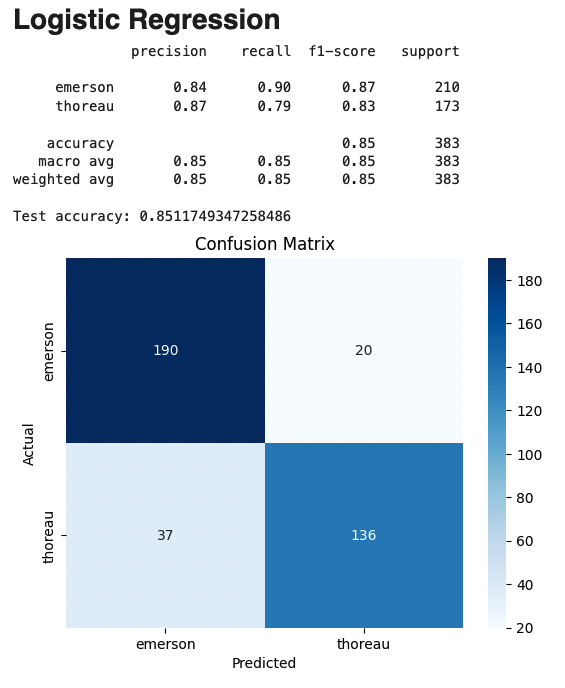
\includegraphics[width=0.75\textwidth]{logistic_regression_confusion.png}

Logistic regression achieves an impressive 85\% accuracy, correctly
identifying the author in most cases.

Here we have included the confusion matrix. For space we will omit this for
most of the models, but they are available in the
\href{https://github.com/ranton256/classifying_concord/tree/main}{GitHub
repo} in the original notebook.

\subsubsection{Random Forest}\label{random-forest}

Next, we implement a Random Forest classifier, which creates an ensemble
of decision trees (Breiman, 2001).

\begin{Shaded}
\begin{Highlighting}[]
\NormalTok{rf }\OperatorTok{=}\NormalTok{ RandomForestClassifier()}
\NormalTok{rf.fit(x\_train, y\_train)}
\NormalTok{y\_pred\_rf }\OperatorTok{=}\NormalTok{ rf.predict(x\_test)}
\end{Highlighting}
\end{Shaded}

Results:

\begin{Shaded}
\begin{Highlighting}[]
\NormalTok{precision    recall  f1{-}score   support}

\NormalTok{emerson       0.82      0.88      0.85       210}
\NormalTok{thoreau       0.84      0.76      0.80       173}

\NormalTok{accuracy                          0.83       383}
\end{Highlighting}
\end{Shaded}

The Random Forest model achieves 83\% accuracy, slightly lower than
logistic regression.

\subsubsection{Support Vector Machine}\label{support-vector-machine}

We also implement a
\href{https://en.wikipedia.org/wiki/Support_vector_machine}{Support
Vector Machine} (SVM) with a radial basis function kernel.
SVM\textquotesingle s are often a strong model compared to traditional
neural networks (pre-transformer,etc) that can train more quickly and
often converge more reliabily (Cortes \& Vapnik 1995). If you are not
familiar with SVMs and want to understand the theory behind them a good
place to start is the KDnuggets article
\href{https://www.kdnuggets.com/2023/07/gentle-introduction-support-vector-machines.html}{\emph{A
gentle introduction to support vector machines}} (Priya, 2023).

\begin{Shaded}
\begin{Highlighting}[]
\NormalTok{clf }\OperatorTok{=}\NormalTok{ svm.SVC(kernel}\OperatorTok{=}\StringTok{\textquotesingle{}rbf\textquotesingle{}}\NormalTok{)}
\NormalTok{clf.fit(x\_train, y\_train)}
\NormalTok{y\_pred\_svm }\OperatorTok{=}\NormalTok{ clf.predict(x\_test)}
\end{Highlighting}
\end{Shaded}

Results:

\begin{Shaded}
\begin{Highlighting}[]
\NormalTok{precision    recall  f1{-}score   support}

\NormalTok{emerson       0.84      0.90      0.87       210}
\NormalTok{thoreau       0.87      0.80      0.83       173}

\NormalTok{accuracy                          0.86       383}
\end{Highlighting}
\end{Shaded}

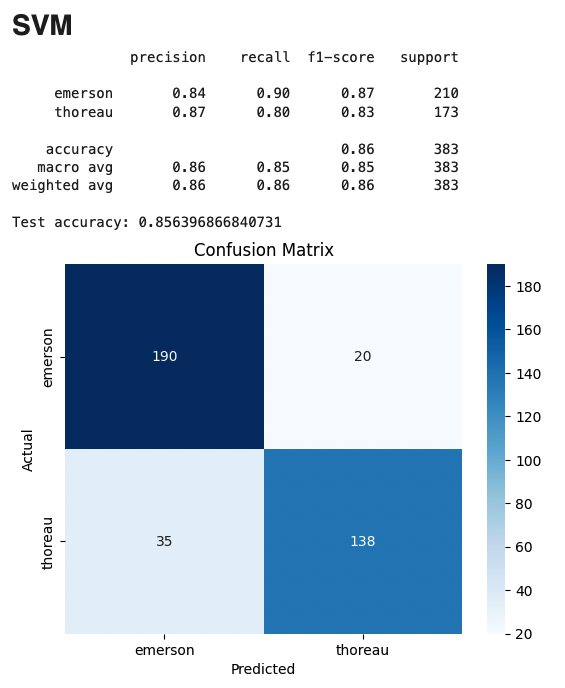
\includegraphics[width=0.75\textwidth]{svm_confusion.png}

The SVM achieves our best traditional model performance at 86\%
accuracy. I think SVM\textquotesingle s are somewhat underappreciated
amid all the neural network hype, for reference on this see
"\href{https://dl.acm.org/doi/10.5555/2627435.2697065}{Do we Need
Hundreds of Classifiers to Solve Real World Classification Problems?}"
by Fernández-Delgado et al. (2014). SVMs can be trained in an amount of
time that is quite zippy compared to more complex models that do not
always beat them without a lot of training data and with less risk of
overfitting.

\subsection{Deep Learning and Transformer
Models}\label{deep-learning-and-transformer-models}

Transformer models revolutionized NLP tasks by capturing complex
contextual relationships in text (Wolf et al., 2020). Here we use
DistilBERT (Sanh, Debut, Chaumond, \& Wolf, 2019), a lightweight version
of BERT (Bidirectional Encoder Representations from Transformers)
(Devlin, Chang, Lee, \& Toutanova, 2019). We use the popular
\href{https://github.com/huggingface/transformers}{Tranformers} open
source library (Wolf et al., 2020) from
\href{https://huggingface.co/}{Hugging Face} for loading, training, and running the model.

Unlike traditional methods that treat words as independent units,
transformer models like BERT understand context by analyzing how words
relate to all other words in a sentence simultaneously. This
\textquotesingle attention mechanism\textquotesingle{} allows the model
to capture subtle stylistic patterns that might be missed by simpler
approaches.

In 2025, DistilBERT is not exactly state of the art, however you can
train or fine-tune it easily with very modest resources. You can replicate this entire project in Google Colab for free.

We employ two different strategies using DistilBERT:

\begin{enumerate}
\def\labelenumi{\arabic{enumi}.}
\item
  \textbf{Feature Extraction}: We freeze DistilBERT\textquotesingle s
  pre-trained weights and use its internal representations as
  sophisticated features for a traditional classifier.
\item
  \textbf{Fine-tuning}: We allow DistilBERT\textquotesingle s weights to
  update during training on our dataset, adapting the entire model
  specifically for our Emerson vs. Thoreau classification task.
\end{enumerate}

\subsubsection{Feature Extraction
Approach}\label{feature-extraction-approach}

First, we use DistilBERT as a feature extractor, employing its hidden
states as input to traditional classifiers. This method is useful in
situations where you may not have enough data to effectively train a
model from scratch, but you want something more powerful than simple
feature engineering techniques.

\begin{Shaded}
\begin{Highlighting}[]
\NormalTok{tokenizer }\OperatorTok{=}\NormalTok{ AutoTokenizer.from\_pretrained(}\StringTok{"distilbert{-}base{-}uncased"}\NormalTok{)}
\NormalTok{model }\OperatorTok{=}\NormalTok{ AutoModel.from\_pretrained(}\StringTok{"distilbert{-}base{-}uncased"}\NormalTok{)}

\CommentTok{\# Tokenize text and get hidden states}
\ControlFlowTok{with}\NormalTok{ torch.no\_grad():}
\NormalTok{    hidden\_train }\OperatorTok{=}\NormalTok{ model(}\OperatorTok{**}\NormalTok{x\_train\_tok)}
\NormalTok{    hidden\_test }\OperatorTok{=}\NormalTok{ model(}\OperatorTok{**}\NormalTok{x\_test\_tok)}
    \CommentTok{\# Get the [CLS] hidden states}
\NormalTok{    cls\_train }\OperatorTok{=}\NormalTok{ hidden\_train.last\_hidden\_state[:,}\DecValTok{0}\NormalTok{,:]}
\NormalTok{    cls\_test }\OperatorTok{=}\NormalTok{ hidden\_test.last\_hidden\_state[:,}\DecValTok{0}\NormalTok{,:]}
\end{Highlighting}
\end{Shaded}

There is a fair bit of code we are leaving out of the article to get
things in a form to make the Transformers library happy here since
everything before this point was setup with scikit learn.

We then use these features with our traditional classifiers:

\textbf{Logistic Regression on DistilBERT hidden states}:

\begin{Shaded}
\begin{Highlighting}[]
\NormalTok{precision    recall  f1{-}score   support}

\NormalTok{emerson       0.91      0.91      0.91       210}
\NormalTok{thoreau       0.90      0.89      0.89       173}

\NormalTok{accuracy                          0.90       383}
\end{Highlighting}
\end{Shaded}

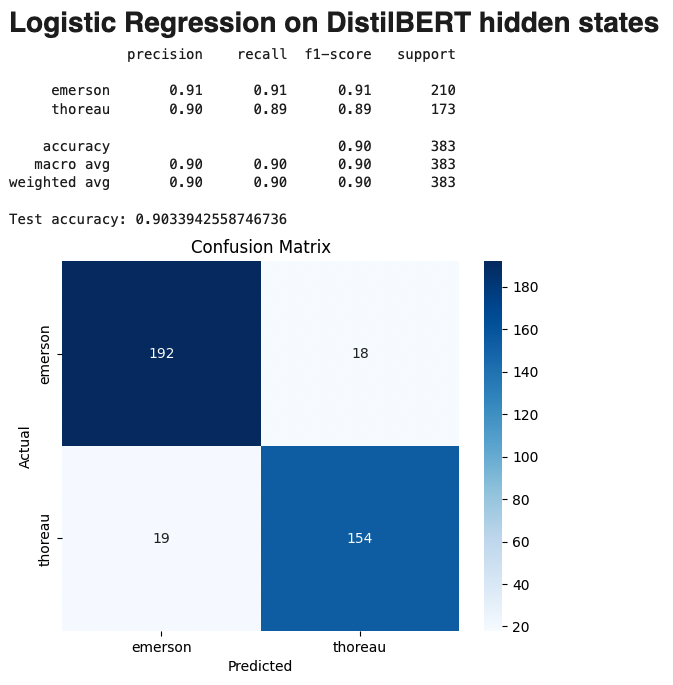
\includegraphics[width=0.75\textwidth]{lr_dbert_confusion.png}

\textbf{SVM on DistilBERT hidden states}:

\begin{Shaded}
\begin{Highlighting}[]
\NormalTok{precision    recall  f1{-}score   support}

\NormalTok{emerson       0.88      0.92      0.90       210}
\NormalTok{thoreau       0.90      0.85      0.87       173}

\NormalTok{accuracy                          0.89       383}
\end{Highlighting}
\end{Shaded}

This hybrid approach shows a significant improvement, with accuracy
increasing to 90\%.

\subsubsection{Fine-tuning DistilBERT}\label{fine-tuning-distilbert}

And finally, we
\href{https://huggingface.co/docs/transformers/en/training}{fine-tune}
DistilBERT specifically for our classification task using the training split of our dataset.

\begin{Shaded}
\begin{Highlighting}[]
\ImportTok{from}\NormalTok{ transformers }\ImportTok{import}\NormalTok{ DistilBertForSequenceClassification}

\NormalTok{model }\OperatorTok{=}\NormalTok{ DistilBertForSequenceClassification.from\_pretrained(}
    \StringTok{\textquotesingle{}distilbert{-}base{-}uncased\textquotesingle{}}\NormalTok{, num\_labels}\OperatorTok{=}\DecValTok{2}
\NormalTok{)}

\CommentTok{\# create our optimizer}
\ImportTok{from}\NormalTok{ torch.optim }\ImportTok{import}\NormalTok{ AdamW}

\NormalTok{optimizer }\OperatorTok{=}\NormalTok{ AdamW(model.parameters(), lr}\OperatorTok{=}\FloatTok{5e{-}5}\NormalTok{)}
\CommentTok{\# a bunch of stuff for preprocessing you can find in GitHub...}
\end{Highlighting}
\end{Shaded}

Here we have left out a bunch of preprocessing code and other boiler
plate for brevity which you can find in the repo.

\begin{Shaded}
\begin{Highlighting}[]
\ImportTok{from}\NormalTok{ transformers }\ImportTok{import}\NormalTok{ Trainer, TrainingArguments, DataCollatorWithPadding}

\NormalTok{data\_collator }\OperatorTok{=}\NormalTok{ DataCollatorWithPadding(tokenizer}\OperatorTok{=}\NormalTok{tokenizer)}

\NormalTok{training\_args }\OperatorTok{=}\NormalTok{ TrainingArguments(}
\NormalTok{    output\_dir}\OperatorTok{=}\StringTok{"./results"}\NormalTok{,}
\NormalTok{    learning\_rate}\OperatorTok{=}\FloatTok{2e{-}4}\NormalTok{,}
\NormalTok{    per\_device\_train\_batch\_size}\OperatorTok{=}\DecValTok{8}\NormalTok{,}
\NormalTok{    per\_device\_eval\_batch\_size}\OperatorTok{=}\DecValTok{8}\NormalTok{,}
\NormalTok{    num\_train\_epochs}\OperatorTok{=}\DecValTok{5}\NormalTok{,}
\NormalTok{    weight\_decay}\OperatorTok{=}\FloatTok{0.01}\NormalTok{,}
\NormalTok{    evaluation\_strategy}\OperatorTok{=}\StringTok{"epoch"}\NormalTok{,}
\NormalTok{    logging\_strategy}\OperatorTok{=}\StringTok{"epoch"}
\NormalTok{)}

\CommentTok{\# Define Trainer object for training the model}
\NormalTok{trainer }\OperatorTok{=}\NormalTok{ Trainer(}
\NormalTok{    model}\OperatorTok{=}\NormalTok{model,}
\NormalTok{    args}\OperatorTok{=}\NormalTok{training\_args,}
\NormalTok{    train\_dataset}\OperatorTok{=}\NormalTok{tokenized\_train,}
\NormalTok{    eval\_dataset}\OperatorTok{=}\NormalTok{tokenized\_test,}
\NormalTok{    tokenizer}\OperatorTok{=}\NormalTok{tokenizer,}
\NormalTok{    data\_collator}\OperatorTok{=}\NormalTok{data\_collator,}
\NormalTok{)}

\NormalTok{trainer.train()}
\end{Highlighting}
\end{Shaded}

Results:

\begin{Shaded}
\begin{Highlighting}[]
\NormalTok{precision    recall  f1{-}score   support}

\NormalTok{emerson       0.93      0.93      0.93       210}
\NormalTok{thoreau       0.91      0.91      0.91       173}

\NormalTok{accuracy                          0.92       383}
\end{Highlighting}
\end{Shaded}

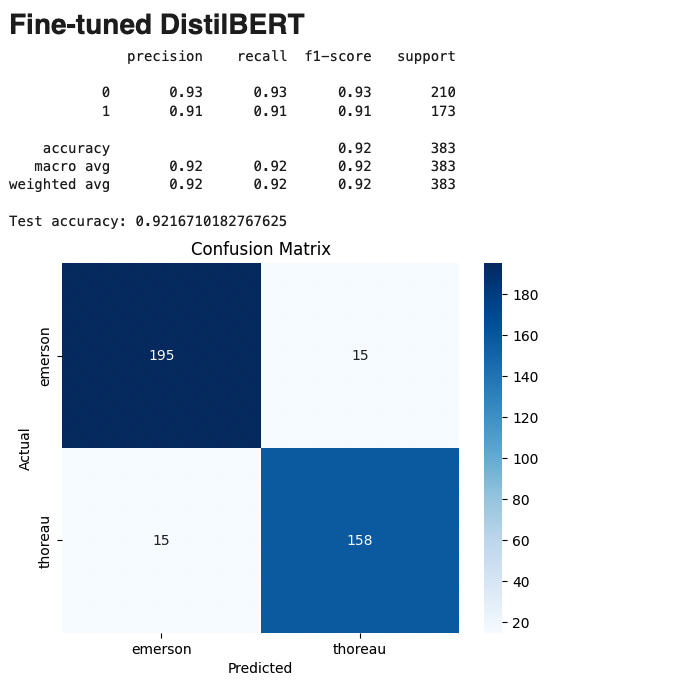
\includegraphics[width=0.75\textwidth]{fine_tuned_dbert_confusion.png}

The fine-tuned DistilBERT achieves our best performance at 92\%
accuracy, demonstrating how powerful transformer models are for
capturing subtle stylistic differences.

\subsection{Analysis of Results}\label{analysis-of-results}

\subsubsection{Performance Comparison}\label{performance-comparison}

Looking at our results across models:

\begin{enumerate}
\def\labelenumi{\arabic{enumi}.}
\item
  Traditional ML models (TF-IDF + classifiers): 83-86\% accuracy
\item
  DistilBERT features + traditional classifiers: 89-90\% accuracy
\item
  Fine-tuned DistilBERT: 92\% accuracy
\end{enumerate}

This progression demonstrates the advantages of modern transformer
models, which capture contextual information and semantic relationships
beyond what bag-of-words approaches can represent.

The 6-9\% accuracy improvement from traditional ML to transformers
suggests that author style involves subtle contextual patterns beyond
simple word frequency that require more sophisticated language
understanding to detect.

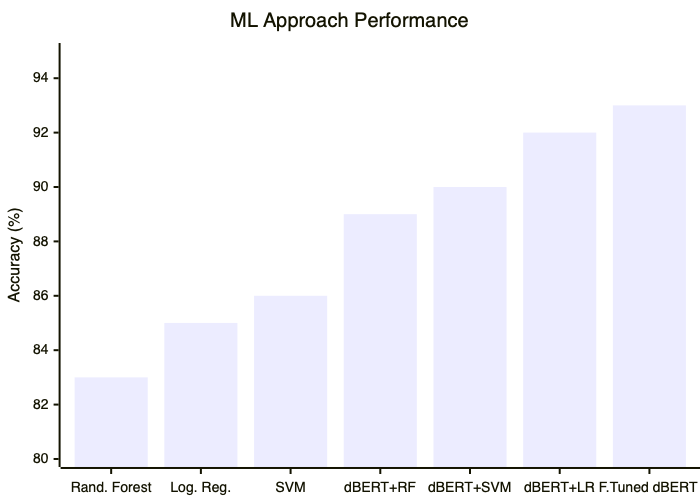
\includegraphics[width=0.95\textwidth,height=\textheight]{image-20250611165131238.png}

\subsubsection{Misclassification
Analysis}\label{misclassification-analysis}

Examining misclassified examples provides some insights on model performance relative to different aspects of input samples:

\begin{Shaded}
\begin{Highlighting}[]
\ControlFlowTok{for}\NormalTok{ i, (txt, lbl, pred) }\KeywordTok{in} \BuiltInTok{enumerate}\NormalTok{(}\BuiltInTok{zip}\NormalTok{(x\_test\_trans, y\_test\_trans, y\_pred\_trans)):}
    \ControlFlowTok{if}\NormalTok{ lbl }\OperatorTok{!=}\NormalTok{ pred:}
        \BuiltInTok{print}\NormalTok{(}\SpecialStringTok{f"}\SpecialCharTok{\{}\NormalTok{lbl}\OperatorTok{=}\SpecialCharTok{\}}\SpecialStringTok{,}\SpecialCharTok{\{}\NormalTok{pred}\OperatorTok{=}\SpecialCharTok{\}}\SpecialStringTok{"}\NormalTok{)}
\NormalTok{        row }\OperatorTok{=}\NormalTok{(my\_cat\_labels[lbl], my\_cat\_labels[pred], txt)}
\NormalTok{        rows.append(row)}
\end{Highlighting}
\end{Shaded}

Several patterns emerge in the 30 misclassified examples (out of 383):

\begin{enumerate}
\def\labelenumi{\arabic{enumi}.}
\item
  \textbf{Project Gutenberg boilerplate}: Many misclassifications
  involve similar license text that appears in both works
\item
  \textbf{Short segments}: Brief text snippets provide insufficient
  stylistic markers
\item
  \textbf{Universal themes}: When both authors discuss similar
  philosophical concepts, the distinction blurs
\item
  \textbf{Quotations}: When either author quotes someone else, their
  personal style is diminished.
\end{enumerate}

One interesting observation is that Thoreau\textquotesingle s more
practical descriptions seem to rarely be misclassified, while his philosophical
musings more frequently get attributed to Emerson. This aligns with our
understanding of their writing styles-Thoreau\textquotesingle s
concrete observations of nature are distinctive, while both authors
share transcendentalist philosophical language.

It is also interesting to look at the length of passages versus the
author prediction correctness.

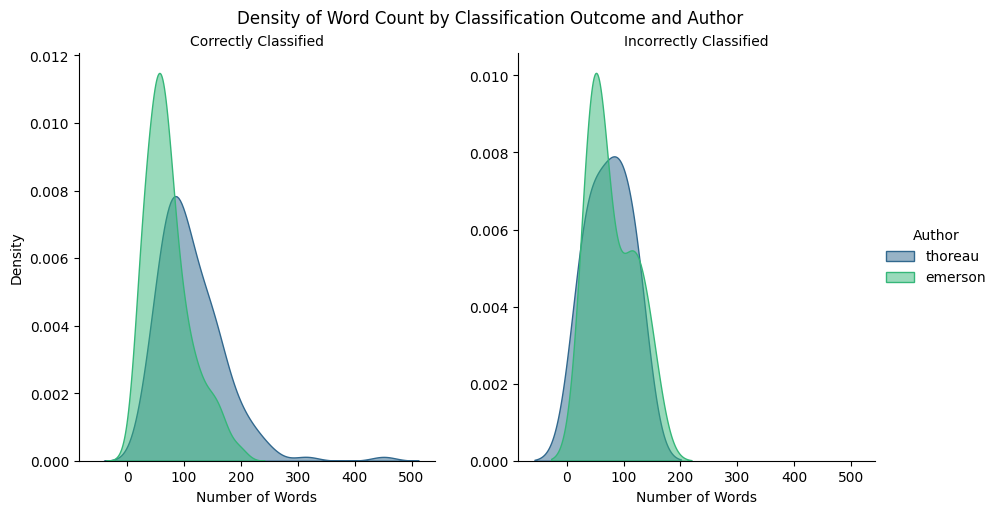
\includegraphics{density_plots.png}

\textbf{Word Count (Median/Average)}

\begin{longtable}[]{@{}lll@{}}
\toprule\noalign{}
Classification & Correctly Classified & Incorrectly Classified \\
\midrule\noalign{}
\endhead
\bottomrule\noalign{}
\endlastfoot
all & 78.00/90.59 & 68.50/77.50 \\
thoreau & 100.00/111.79 & 78.50/74.38 \\
emerson & 62.00/71.52 & 65.50/79.06 \\
\end{longtable}

We can see that the median and average length correleates significantly
with correctness for passages by Thoreau but seems to have less relation
for passages by Emerson.

\subsubsection{Model Interpretability}\label{model-interpretability}

While transformer models achieve the highest accuracy, they function as
"black boxes" compared to traditional models. With logistic regression,
we can examine the coefficients to identify the most influential words
for classification:

The most strongly Emerson-associated terms include abstract nouns and
adjectives like "soul," "divine," "intellect," and "universal."
Thoreau\textquotesingle s distinctive vocabulary includes more concrete
terms like "pond," "woods," "house," and action verbs reflecting his
practical experiences at Walden.

\subsection{Conclusion}\label{conclusion}

The results show how well even simpler ML models can distinguish between the literary style of these two authors. The fine-tuned DistilBERT model achieved 92\% accuracy on the test set, while traditional machine learning approaches reached 83–86\% accuracy.

The performance progression from traditional to transformer-based models reflects broader developments in natural language processing. TF-IDF vectorization with classic algorithms provided a functional baseline (83–86\% accuracy), while transformer models improved on these results (92\% accuracy) by capturing contextual relationships between words.

The misclassification analysis revealed some specific patterns in the 30 misclassified examples (from 383 total test examples). These conclusions are qualitative and somewhat subjective, but indicate a tendency for quotations, shorter samples, and topic to affect the accuracy of the model on particular samples.

The classification results highlight the distinct writing styles of that Emerson and Thoreau despite their shared historical context, philosophy, interests, and proximity.

If you made it here thanks for reading, and I hope you found this helpful and interesting.

\subsection{Project Repository}\label{project-repository}

All code is available at https://github.com/ranton256/classifying\_concord

\subsection{References}\label{references}

\subsubsection{Literary Works and
Sources}\label{literary-works-and-sources}

\begin{enumerate}
\def\labelenumi{\arabic{enumi}.}
\item
  Emerson, R.W. (1841). \emph{Essays: First Series}. James Munroe and
  Company. Retrieved from Project Gutenberg:
  \url{https://www.gutenberg.org/ebooks/16643}
\item
  Gross, R. A. (2021).
  \href{https://us.macmillan.com/books/9780374279325/thetranscendentalistsandtheirworld/}{\emph{The
  transcendentalists and their world}}. Farrar, Straus and Giroux.
\item
  Thoreau, H.D. (1854). \emph{Walden, and On The Duty Of Civil
  Disobedience}. Ticknor and Fields. Retrieved from Project Gutenberg:
  \url{https://www.gutenberg.org/ebooks/205}
\item
  Richardson, R.D. (1995). \emph{Emerson: The Mind on Fire}. University
  of California Press.
\item
  Walls, L.D. (2017). \emph{Henry David Thoreau: A Life}. University of
  Chicago Press.
\item
  Buell, L. (2003). \emph{Emerson}. Harvard University Press.
\end{enumerate}

\subsubsection{Machine Learning and NLP
References}\label{machine-learning-and-nlp-references}

\begin{enumerate}
\def\labelenumi{\arabic{enumi}.}
\item
  Breiman, L. (2001). Random Forests. \emph{Machine Learning, 45}, 5-32.
  \url{https://doi.org/10.1023/A:1010933404324}
\item
  Cortes, C., \& Vapnik, V.N. (1995). Support-Vector Networks.
  \emph{Machine Learning, 20},
  273-297.\url{https://doi.org/10.1007/BF00994018}
\item
  Cox, David R. (1958). "The regression analysis of binary sequences
  (with discussion)". \emph{J R Stat Soc B}. 20 (2): 215--242.
  \url{https://doi.org/10.1111\%2Fj.2517-6161.1958.tb00292.x}.
  \href{https://en.wikipedia.org/wiki/JSTOR_(identifier)}{JSTOR}
  \href{https://www.jstor.org/stable/2983890}{2983890}.
\item
  Devlin, J., Chang, M.W., Lee, K., \& Toutanova, K. (2019). BERT:
  Pre-training of Deep Bidirectional Transformers for Language
  Understanding. \emph{Proceedings of NAACL-HLT 2019}, 4171--4186.
  \url{https://doi.org/10.18653/v1/N19-1423}
\item
  Hastie, T., Tibshirani, R., \& Friedman, J. (2009). \emph{The Elements
  of Statistical Learning: Data Mining, Inference, and Prediction} (2nd
  ed.). Springer.
\item
  Honnibal, M., \& Montani, I. (2017). spaCy 2: Natural language
  understanding with Bloom embeddings, convolutional neural networks and
  incremental parsing.
\item
  Jayaswal, V. (2020, September 14). \emph{Performance metrics:
  Confusion matrix, precision, recall, and F1 score}. Towards Data
  Science.
  \url{https://towardsdatascience.com/performance-metrics-confusion-matrix-precision-recall-and-f1-score-a8fe076a2262/}
\item
  Pedregosa, F., Varoquaux, G., Gramfort, A., Michel, V., Thirion, B.,
  Grisel, O., ... \& Duchesnay, É. (2011). Scikit-learn: Machine
  Learning in Python. \emph{Journal of Machine Learning Research}, 12,
  2825-2830.
\item
  Priya, B. C. (2023, July 10). \emph{A gentle introduction to support
  vector machines}. KDnuggets.
  \url{https://www.kdnuggets.com/2023/07/gentle-introduction-support-vector-machines.html}
\item
  Sanh, V., Debut, L., Chaumond, J., \& Wolf, T. (2019). DistilBERT, a
  distilled version of BERT: smaller, faster, cheaper and lighter.
  \emph{ArXiv, abs/1910.01108}.
  \url{https://doi.org/10.48550/arXiv.1910.01108}
\item
  Sebastiani, F. (2002). Machine learning in automated text
  categorization. \emph{ACM Computing Surveys}, 34(1), 1--47.
  \url{https://doi.org/10.1145/505282.505283}
\item
  Spärck Jones, K. (1973). Index term weighting. \emph{Inf. Storage
  Retr., 9}, 619-633.
\item
  Vaswani, A., Shazeer, N.M., Parmar, N., Uszkoreit, J., Jones, L.,
  Gomez, A.N., Kaiser, L., \& Polosukhin, I. (2017).
  \href{https://arxiv.org/abs/1706.03762}{Attention is All you Need.}
  \emph{Neural Information Processing Systems}.
\item
  Wolf, T., Debut, L., Sanh, V., Chaumond, J., Delangue, C., Moi, A.,
  ... \& Rush, A. M. (2020). Transformers: State-of-the-Art Natural
  Language Processing. \emph{Proceedings of the 2020 Conference on
  Empirical Methods in Natural Language Processing: System
  Demonstrations}, 38--45.
\end{enumerate}

\subsubsection{Computational Stylometry and Literary
Analysis}\label{computational-stylometry-and-literary-analysis}

\begin{enumerate}
\def\labelenumi{\arabic{enumi}.}
\item
  Burrows, J. (2002). \textquotesingle Delta\textquotesingle: a Measure
  of Stylistic Difference and a Guide to Likely Authorship.
  \emph{Literary and Linguistic Computing}, 17(3), 267--287.
  \url{https://doi.org/10.1093/llc/17.3.267}
\item
  Jockers, M.L. (2013). \emph{Macroanalysis: Digital Methods and
  Literary History}. University of Illinois Press.
\item
  Stamatatos, E. (2009). A survey of modern authorship attribution
  methods. \emph{Journal of the American Society for Information Science
  and Technology}, 60(3), 538-556.
  \url{https://doi.org/10.1002/asi.21001}
\item
  Underwood, T. (2019). \emph{Distant Horizons: Digital Evidence and
  Literary Change}. University of Chicago Press.
\end{enumerate}

\subsubsection{Python Libraries and
Tools}\label{python-libraries-and-tools}

\begin{enumerate}
\def\labelenumi{\arabic{enumi}.}
\item
  Pandas Development Team (2020). pandas-dev/pandas: Pandas. Zenodo.
  \url{https://doi.org/10.5281/zenodo.3509134}
\item
  Harris, C.R., Millman, K.J., van der Walt, S.J. et al. (2020). Array
  programming with NumPy. \emph{Nature}, 585, 357--362.
  \url{https://doi.org/10.1038/s41586-020-2649-2}
\item
  Hunter, J. D. (2007). Matplotlib: A 2D Graphics Environment.
  \emph{Computing in Science \& Engineering}, 9(3), 90-95.
  \url{https://doi.org/10.1109/MCSE.2007.55}
\item
  Pedregosa \emph{et al.} (2011).
  \href{https://scikit-learn.org/}{Scikit-learn}: Machine Learning in
  Python. \emph{Journal of Machine Learning Research}, \emph{12},
  2825--2830.
\item
  Waskom, M.L. (2021). seaborn: statistical data visualization.
  \emph{Journal of Open Source Software}, 6(60), 3021.
  \url{https://doi.org/10.21105/joss.03021}
\item
  Paszke, A., Gross, S., Massa, F., Lerer, A., Bradbury, J., Chanan, G.,
  ... \& Chintala, S. (2019). PyTorch: An Imperative Style,
  High-Performance Deep Learning Library. \emph{Advances in Neural
  Information Processing Systems}, 32, 8026-8037.
\end{enumerate}

\subsubsection{Core NLP and Text
Classification}\label{core-nlp-and-text-classification}

\begin{itemize}
\item
  Fernández-Delgado, M., Cernadas, E., Barro, S., \& Amorim, D. (2014).
  Do we need hundreds of classifiers to solve real world classification
  problems? Journal of Machine Learning Research, 15(1), 3133-3181.
\item
  Hochreiter, S., \& Schmidhuber, J. (1997). Long short-term memory.
  Neural computation, 9(8), 1735-1780.
\item
  Koppel, M., Schler, J., \& Argamon, S. (2009). Computational methods
  in authorship attribution. Journal of the American Society for
  Information Science and Technology, 60(1), 9-26.
\item
  LeCun, Y., Bottou, L., Bengio, Y., \& Haffner, P. (1998).
  Gradient-based learning applied to document recognition. Proceedings
  of the IEEE, 86(11), 2278-2324.
\item
  Manning, C. D., \& Schütze, H. (1999). Foundations of statistical
  natural language processing. MIT Press.
\item
  Project Gutenberg. (n.d.). Free eBooks.
  \url{https://www.gutenberg.org/}
\item
  Rocchio Jr, J. J. (1971). Relevance feedback in information retrieval.
  The SMART retrieval system: experiments in automatic document
  processing, 313-323.
\item
  Wolf, T., Debut, L., Sanh, V., Chaumond, J., Delangue, C., Moi, A.,
  Cistac, P., Rault, T., Louf, R., Funtowicz, M., Davison, J., Shleifer,
  S., Platen, P.V., Ma, C., Jernite, Y., Plu, J., Xu, C., Scao, T.L.,
  Gugger, S., Drame, M., Lhoest, Q., \& Rush, A.M. (2020).
  \href{https://aclanthology.org/2020.emnlp-demos.6/}{Transformers:
  State-of-the-Art Natural Language Processing.} \emph{Conference on
  Empirical Methods in Natural Language Processing}.
\item
  Salton, G., \& Buckley, C. (1988). Term-weighting approaches in
  automatic text retrieval. Information processing \& management, 24(5),
  513-523.
\item
  Spärck Jones, K. (1972). A statistical interpretation of term
  specificity and its application in retrieval. Journal of
  documentation, 28(1), 11-21.
\end{itemize}

\end{document}